% --------------------------------------------------------------
% This is all preamble stuff that you don't have to worry about.
% Head down to where it says "Start here"
% --------------------------------------------------------------
 
\documentclass[12pt]{article}
 
\usepackage[margin=1in]{geometry} 
\usepackage{amsmath,amsthm,amssymb}
\usepackage{graphicx}
 

\begin{document}
 
% --------------------------------------------------------------
%                         Start here
% --------------------------------------------------------------
 
\title{Practical No. 1 }%replace X with the appropriate number
\author{Tomasz Siłkowski
ts407106@students.mimuw.edu.pl}
 
\maketitle
 
\section{Part 1 }
\subsection*{a) }
In Figure 1 we can see that all occupations are clustered together, which is
pleasing. However, we can see that 'literatura' is so close to occupations 
that it could be mistaken as one.

\begin{figure}[!h]
\centering
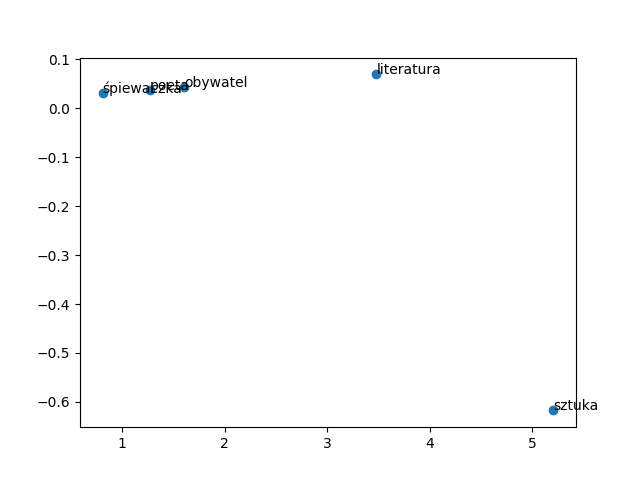
\includegraphics[width=0.95\columnwidth]{plot_1e_1.png}
\caption{Normalized Polish corpus vector space}
\label{fig:image}
\end{figure}

\subsection*{b) }
In Figure 2 there's a similar situation: occupations are well clustered,
while 'sztuka' is correctly distanced. Problem with 'literatura' has lessened,
but I think it should be closer to 'sztuka' compared to the occupations still.

\begin{figure}[!h]
\centering
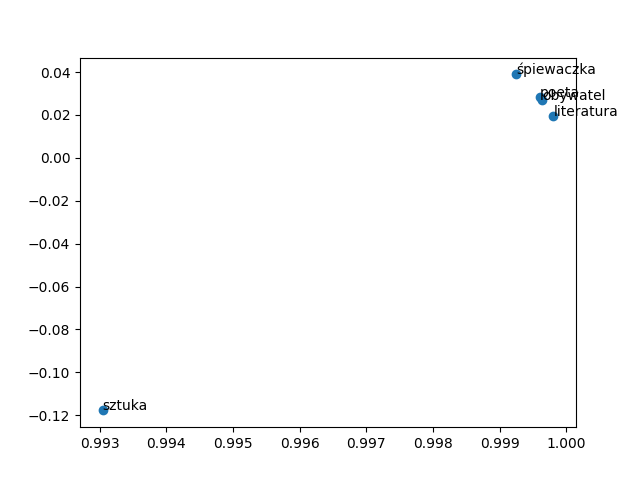
\includegraphics[width=0.95\columnwidth]{plot_1e_2.png}
\caption{Unnormalized Polish corpus vector space}
\label{fig:image}
\end{figure}

 
\section{Prediction-Based Word Vectors in Polish Corpus}
\subsection*{a) Reducing dimensionality of Word2Vec Word Embeddings}

\begin{figure}[!h]
\centering
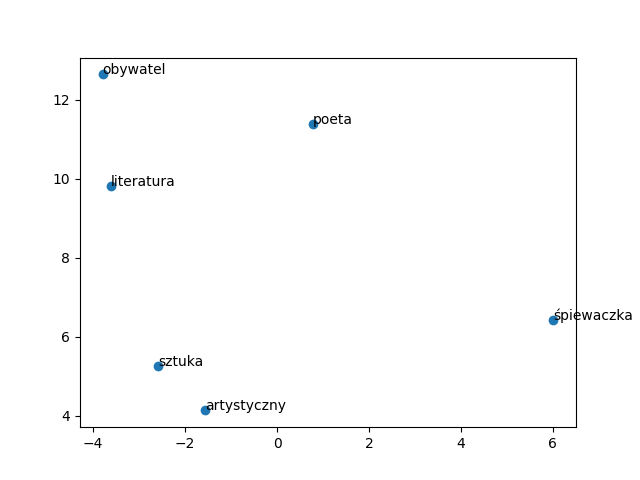
\includegraphics[width=0.95\columnwidth]{plot_2a.png}
\caption{Polish corpus vector space with reduced dimensionality}
\label{fig:image}
\end{figure}

Figure 3 shows that, after reducing dimensionality, most of sample words are 
quite spaced out, we see new relations such as 'sztuka' close to 'artystyczny', 
however words denoting occupations ('poeta' and 'śpiewaczka') are quite far away.

\subsection*{b) Polysemous words}
Example of a polysemous word I found was 'guzik': in most similar words, it had 
both 'przycisk', alluding to a keyboard or a panel, and 'pasek', which is much 
closer to its meaning in tayloring.

\subsection*{c) Synonyms and Antonyms}
An example of antonyms that are closer than synonyms is 'czysty', 'szlachetny' 
and 'brudny'. I believe that word 'czysty' is much more frequently associated 
with physical state of cleanliness, while ideas of noblity are quite archaic.

\subsection*{d) Finding Analogies}
An analogy I found was 'pociąg':'dworzec' :: 'samolot':'lotnisko'. \\
I think that similarity lays in that trains stop on railway stations and planes 
stop on airports.

\subsection*{e) Incorrect Analogies}
An analogy I found was 'człowiek':'dom' :: 'pies':'kurnik'. \\
Dogs are not housed in chicken coops. Clearly, 'buda' would be much more appropriate.

\subsection*{f) Guided Analysis of Bias in Word Vectors}
In the top 10 most similar results, we find 'agent' and 'wiceprezes', which 
suggests that words representing women are further away from words representing 
leadership roles.

\subsection*{g) Independent Analysis of Bias in Word Vectors}
In the same vein as the example in subsection f, most analogous word to fit in 
'mężczyzna':'garaż' :: 'kobieta':'X', according to the model, is 'pralnia', 
which reveales some unsettlingly sexist relations in the data.

\subsection*{h) The source of bias in word vectors}
The model in this example is assinging each word a point, but there are some 
words which don't have such singular meaning -- for example, some words are for 
both genders. In such situations, model has to compromise and choose the value 
that is more frequent, which often reveales bias of how the word is used on the 
original corpus. Additionally, Polish corpus seems to be more limited in volume 
in comparison to the English one.



\section{Prediction-Based Word Vectors in English Corpus}
\subsection*{b) Polysemous words}
Example of a polysemous word I found was 'free': in most similar words, it had 
both 'restricted', alluding to freedom, and 'nominal fee', which is much 
closer to its meaning as a price.

\subsection*{c) Synonyms and Antonyms}
An example of antonyms that are closer than synonyms is 'smart', 'wise' 
and 'dull'. I believe that word 'smart' is much more frequently associated with 
being sharp and exciting and its meaning corresponding to intelligence is used 
less often.

\subsection*{d) Finding Analogies}
An analogy I found was 'plane':'airport' :: 'ship':'docks'. \\
I think that similarity lays in that planes stop on airports and ships stop in 
docks.

\subsection*{e) Incorrect Analogies}
An analogy I found was 'human':'apartment' :: 'dog':'chinatown'. \\
This is just a stereotype.

\subsection*{f) Guided Analysis of Bias in Word Vectors}
In the top 10 most similar results, we find 'receptionist' and 'coworker', which 
suggests that words representing women are further away from words representing 
leadership roles.

\subsection*{g) Independent Analysis of Bias in Word Vectors}
In the same vein as the example in subsection f, most analogous word to fit in 
'man':'blue' :: 'woman':'X', according to the model, is 'pink'. I do not think 
this is offensive, but it does show that model learned some stereotypes.

\subsection*{h) The source of bias in word vectors}
The model in this example is assinging each word a point, but there are some 
words which don't have such singular meaning -- for example, some words are for 
both genders. In such situations, model has to compromise and choose the value 
that is more frequent, which often reveales bias of how the word is used on the 
original corpus.
 
% --------------------------------------------------------------
%     You don't have to mess with anything below this line.
% --------------------------------------------------------------
 
\end{document}